% Created by tikzDevice version 0.12.3.1 on 2022-08-18 15:37:32
% !TEX encoding = UTF-8 Unicode
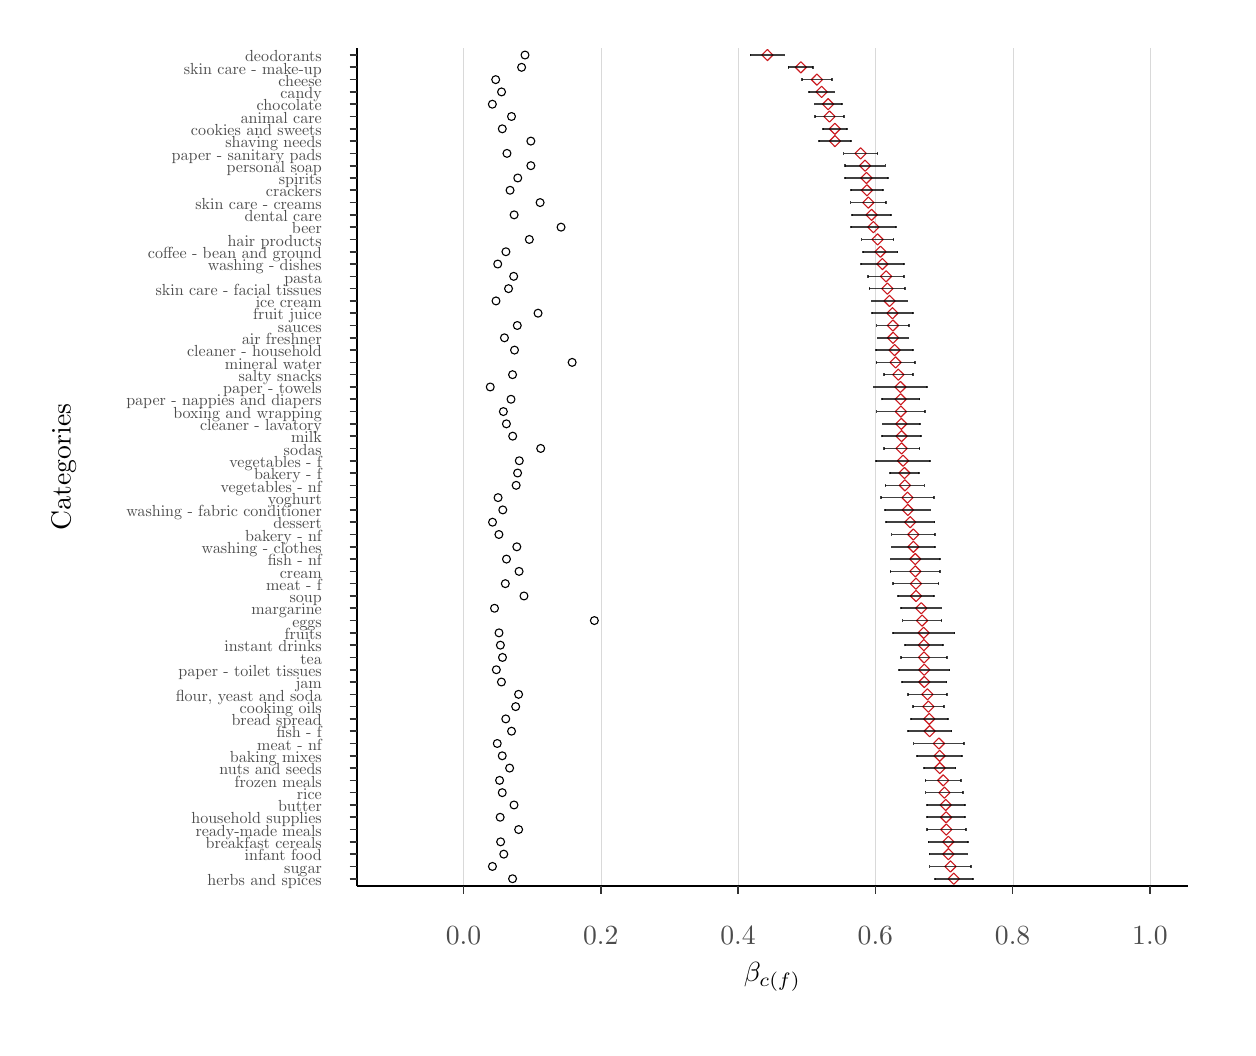
\begin{tikzpicture}[x=1pt,y=1pt]
\definecolor{fillColor}{RGB}{255,255,255}
\path[use as bounding box,fill=fillColor,fill opacity=0.00] (0,0) rectangle (433.62,361.35);
\begin{scope}
\path[clip] (  0.00,  0.00) rectangle (433.62,361.35);
\definecolor{drawColor}{RGB}{255,255,255}
\definecolor{fillColor}{RGB}{255,255,255}

\path[draw=drawColor,line width= 0.6pt,line join=round,line cap=round,fill=fillColor] (  0.00,  0.00) rectangle (433.62,361.35);
\end{scope}
\begin{scope}
\path[clip] (119.04, 51.15) rectangle (419.17,354.12);
\definecolor{drawColor}{RGB}{255,255,255}

\path[draw=drawColor,line width= 0.3pt,line join=round] (132.68, 51.15) --
	(132.68,354.12);

\path[draw=drawColor,line width= 0.3pt,line join=round] (182.29, 51.15) --
	(182.29,354.12);

\path[draw=drawColor,line width= 0.3pt,line join=round] (231.90, 51.15) --
	(231.90,354.12);

\path[draw=drawColor,line width= 0.3pt,line join=round] (281.51, 51.15) --
	(281.51,354.12);

\path[draw=drawColor,line width= 0.3pt,line join=round] (331.11, 51.15) --
	(331.11,354.12);

\path[draw=drawColor,line width= 0.3pt,line join=round] (380.72, 51.15) --
	(380.72,354.12);
\definecolor{drawColor}{gray}{0.85}

\path[draw=drawColor,line width= 0.1pt,line join=round] (157.49, 51.15) --
	(157.49,354.12);

\path[draw=drawColor,line width= 0.1pt,line join=round] (207.09, 51.15) --
	(207.09,354.12);

\path[draw=drawColor,line width= 0.1pt,line join=round] (256.70, 51.15) --
	(256.70,354.12);

\path[draw=drawColor,line width= 0.1pt,line join=round] (306.31, 51.15) --
	(306.31,354.12);

\path[draw=drawColor,line width= 0.1pt,line join=round] (355.92, 51.15) --
	(355.92,354.12);

\path[draw=drawColor,line width= 0.1pt,line join=round] (405.52, 51.15) --
	(405.52,354.12);
\definecolor{drawColor}{RGB}{0,0,0}

\path[draw=drawColor,line width= 0.4pt,line join=round,line cap=round] (172.28,249.28) circle (  1.43);

\path[draw=drawColor,line width= 0.4pt,line join=round,line cap=round] (174.83,329.25) circle (  1.43);

\path[draw=drawColor,line width= 0.4pt,line join=round,line cap=round] (177.03,200.42) circle (  1.43);

\path[draw=drawColor,line width= 0.4pt,line join=round,line cap=round] (170.28,178.21) circle (  1.43);

\path[draw=drawColor,line width= 0.4pt,line join=round,line cap=round] (171.48, 98.24) circle (  1.43);

\path[draw=drawColor,line width= 0.4pt,line join=round,line cap=round] (192.73,289.26) circle (  1.43);

\path[draw=drawColor,line width= 0.4pt,line join=round,line cap=round] (171.89,222.63) circle (  1.43);

\path[draw=drawColor,line width= 0.4pt,line join=round,line cap=round] (172.76,111.57) circle (  1.43);

\path[draw=drawColor,line width= 0.4pt,line join=round,line cap=round] (170.90, 67.15) circle (  1.43);

\path[draw=drawColor,line width= 0.4pt,line join=round,line cap=round] (175.74, 80.47) circle (  1.43);

\path[draw=drawColor,line width= 0.4pt,line join=round,line cap=round] (171.23,338.13) circle (  1.43);

\path[draw=drawColor,line width= 0.4pt,line join=round,line cap=round] (169.12,342.57) circle (  1.43);

\path[draw=drawColor,line width= 0.4pt,line join=round,line cap=round] (167.91,333.69) circle (  1.43);

\path[draw=drawColor,line width= 0.4pt,line join=round,line cap=round] (175.92,244.84) circle (  1.43);

\path[draw=drawColor,line width= 0.4pt,line join=round,line cap=round] (172.99,218.19) circle (  1.43);

\path[draw=drawColor,line width= 0.4pt,line join=round,line cap=round] (172.81,280.38) circle (  1.43);

\path[draw=drawColor,line width= 0.4pt,line join=round,line cap=round] (171.50,324.80) circle (  1.43);

\path[draw=drawColor,line width= 0.4pt,line join=round,line cap=round] (176.34,116.01) circle (  1.43);

\path[draw=drawColor,line width= 0.4pt,line join=round,line cap=round] (174.30,302.59) circle (  1.43);

\path[draw=drawColor,line width= 0.4pt,line join=round,line cap=round] (177.56,164.88) circle (  1.43);

\path[draw=drawColor,line width= 0.4pt,line join=round,line cap=round] (175.78,293.71) circle (  1.43);

\path[draw=drawColor,line width= 0.4pt,line join=round,line cap=round] (179.71,351.46) circle (  1.43);

\path[draw=drawColor,line width= 0.4pt,line join=round,line cap=round] (167.97,182.65) circle (  1.43);

\path[draw=drawColor,line width= 0.4pt,line join=round,line cap=round] (204.77,147.11) circle (  1.43);

\path[draw=drawColor,line width= 0.4pt,line join=round,line cap=round] (174.84,107.13) circle (  1.43);

\path[draw=drawColor,line width= 0.4pt,line join=round,line cap=round] (173.01,169.32) circle (  1.43);

\path[draw=drawColor,line width= 0.4pt,line join=round,line cap=round] (177.39,120.45) circle (  1.43);

\path[draw=drawColor,line width= 0.4pt,line join=round,line cap=round] (170.52, 89.36) circle (  1.43);

\path[draw=drawColor,line width= 0.4pt,line join=round,line cap=round] (184.42,258.17) circle (  1.43);

\path[draw=drawColor,line width= 0.4pt,line join=round,line cap=round] (170.32,142.67) circle (  1.43);

\path[draw=drawColor,line width= 0.4pt,line join=round,line cap=round] (181.27,284.82) circle (  1.43);

\path[draw=drawColor,line width= 0.4pt,line join=round,line cap=round] (175.21, 53.82) circle (  1.43);

\path[draw=drawColor,line width= 0.4pt,line join=round,line cap=round] (170.73, 76.03) circle (  1.43);

\path[draw=drawColor,line width= 0.4pt,line join=round,line cap=round] (169.23,262.61) circle (  1.43);

\path[draw=drawColor,line width= 0.4pt,line join=round,line cap=round] (172.04, 62.70) circle (  1.43);

\path[draw=drawColor,line width= 0.4pt,line join=round,line cap=round] (170.81,138.22) circle (  1.43);

\path[draw=drawColor,line width= 0.4pt,line join=round,line cap=round] (171.19,124.90) circle (  1.43);

\path[draw=drawColor,line width= 0.4pt,line join=round,line cap=round] (168.69,151.55) circle (  1.43);

\path[draw=drawColor,line width= 0.4pt,line join=round,line cap=round] (172.59,160.44) circle (  1.43);

\path[draw=drawColor,line width= 0.4pt,line join=round,line cap=round] (169.68,102.69) circle (  1.43);

\path[draw=drawColor,line width= 0.4pt,line join=round,line cap=round] (175.26,213.74) circle (  1.43);

\path[draw=drawColor,line width= 0.4pt,line join=round,line cap=round] (196.74,240.40) circle (  1.43);

\path[draw=drawColor,line width= 0.4pt,line join=round,line cap=round] (174.15, 93.80) circle (  1.43);

\path[draw=drawColor,line width= 0.4pt,line join=round,line cap=round] (174.65,227.07) circle (  1.43);

\path[draw=drawColor,line width= 0.4pt,line join=round,line cap=round] (173.19,315.92) circle (  1.43);

\path[draw=drawColor,line width= 0.4pt,line join=round,line cap=round] (169.35,129.34) circle (  1.43);

\path[draw=drawColor,line width= 0.4pt,line join=round,line cap=round] (167.15,231.51) circle (  1.43);

\path[draw=drawColor,line width= 0.4pt,line join=round,line cap=round] (175.62,271.49) circle (  1.43);

\path[draw=drawColor,line width= 0.4pt,line join=round,line cap=round] (181.83,311.48) circle (  1.43);

\path[draw=drawColor,line width= 0.4pt,line join=round,line cap=round] (177.41, 71.59) circle (  1.43);

\path[draw=drawColor,line width= 0.4pt,line join=round,line cap=round] (171.49, 84.92) circle (  1.43);

\path[draw=drawColor,line width= 0.4pt,line join=round,line cap=round] (175.21,235.96) circle (  1.43);

\path[draw=drawColor,line width= 0.4pt,line join=round,line cap=round] (176.92,253.73) circle (  1.43);

\path[draw=drawColor,line width= 0.4pt,line join=round,line cap=round] (181.82,320.36) circle (  1.43);

\path[draw=drawColor,line width= 0.4pt,line join=round,line cap=round] (185.16,298.15) circle (  1.43);

\path[draw=drawColor,line width= 0.4pt,line join=round,line cap=round] (173.76,267.05) circle (  1.43);

\path[draw=drawColor,line width= 0.4pt,line join=round,line cap=round] (178.48,347.02) circle (  1.43);

\path[draw=drawColor,line width= 0.4pt,line join=round,line cap=round] (185.38,209.30) circle (  1.43);

\path[draw=drawColor,line width= 0.4pt,line join=round,line cap=round] (179.34,155.99) circle (  1.43);

\path[draw=drawColor,line width= 0.4pt,line join=round,line cap=round] (177.09,307.03) circle (  1.43);

\path[draw=drawColor,line width= 0.4pt,line join=round,line cap=round] (167.94, 58.26) circle (  1.43);

\path[draw=drawColor,line width= 0.4pt,line join=round,line cap=round] (171.57,133.78) circle (  1.43);

\path[draw=drawColor,line width= 0.4pt,line join=round,line cap=round] (177.64,204.86) circle (  1.43);

\path[draw=drawColor,line width= 0.4pt,line join=round,line cap=round] (176.51,195.97) circle (  1.43);

\path[draw=drawColor,line width= 0.4pt,line join=round,line cap=round] (176.75,173.76) circle (  1.43);

\path[draw=drawColor,line width= 0.4pt,line join=round,line cap=round] (169.85,275.94) circle (  1.43);

\path[draw=drawColor,line width= 0.4pt,line join=round,line cap=round] (171.68,187.09) circle (  1.43);

\path[draw=drawColor,line width= 0.4pt,line join=round,line cap=round] (169.97,191.53) circle (  1.43);
\definecolor{drawColor}{RGB}{203,24,29}

\path[draw=drawColor,line width= 0.4pt,line join=round,line cap=round] (310.67,249.28) --
	(312.69,251.30) --
	(314.71,249.28) --
	(312.69,247.27) --
	cycle;

\path[draw=drawColor,line width= 0.4pt,line join=round,line cap=round] (287.70,329.25) --
	(289.72,331.26) --
	(291.74,329.25) --
	(289.72,327.23) --
	cycle;

\path[draw=drawColor,line width= 0.4pt,line join=round,line cap=round] (314.81,200.42) --
	(316.82,202.43) --
	(318.84,200.42) --
	(316.82,198.40) --
	cycle;

\path[draw=drawColor,line width= 0.4pt,line join=round,line cap=round] (318.01,178.21) --
	(320.03,180.22) --
	(322.05,178.21) --
	(320.03,176.19) --
	cycle;

\path[draw=drawColor,line width= 0.4pt,line join=round,line cap=round] (327.51, 98.24) --
	(329.53,100.26) --
	(331.55, 98.24) --
	(329.53, 96.23) --
	cycle;

\path[draw=drawColor,line width= 0.4pt,line join=round,line cap=round] (303.57,289.26) --
	(305.59,291.28) --
	(307.61,289.26) --
	(305.59,287.25) --
	cycle;

\path[draw=drawColor,line width= 0.4pt,line join=round,line cap=round] (313.51,222.63) --
	(315.53,224.65) --
	(317.55,222.63) --
	(315.53,220.61) --
	cycle;

\path[draw=drawColor,line width= 0.4pt,line join=round,line cap=round] (323.77,111.57) --
	(325.79,113.59) --
	(327.80,111.57) --
	(325.79,109.55) --
	cycle;

\path[draw=drawColor,line width= 0.4pt,line join=round,line cap=round] (330.66, 67.15) --
	(332.68, 69.16) --
	(334.69, 67.15) --
	(332.68, 65.13) --
	cycle;

\path[draw=drawColor,line width= 0.4pt,line join=round,line cap=round] (329.71, 80.47) --
	(331.73, 82.49) --
	(333.75, 80.47) --
	(331.73, 78.46) --
	cycle;

\path[draw=drawColor,line width= 0.4pt,line join=round,line cap=round] (284.87,338.13) --
	(286.89,340.15) --
	(288.91,338.13) --
	(286.89,336.11) --
	cycle;

\path[draw=drawColor,line width= 0.4pt,line join=round,line cap=round] (283.18,342.57) --
	(285.19,344.59) --
	(287.21,342.57) --
	(285.19,340.56) --
	cycle;

\path[draw=drawColor,line width= 0.4pt,line join=round,line cap=round] (287.22,333.69) --
	(289.24,335.71) --
	(291.26,333.69) --
	(289.24,331.67) --
	cycle;

\path[draw=drawColor,line width= 0.4pt,line join=round,line cap=round] (311.23,244.84) --
	(313.25,246.86) --
	(315.27,244.84) --
	(313.25,242.82) --
	cycle;

\path[draw=drawColor,line width= 0.4pt,line join=round,line cap=round] (313.67,218.19) --
	(315.68,220.20) --
	(317.70,218.19) --
	(315.68,216.17) --
	cycle;

\path[draw=drawColor,line width= 0.4pt,line join=round,line cap=round] (306.12,280.38) --
	(308.14,282.40) --
	(310.16,280.38) --
	(308.14,278.36) --
	cycle;

\path[draw=drawColor,line width= 0.4pt,line join=round,line cap=round] (289.67,324.80) --
	(291.69,326.82) --
	(293.70,324.80) --
	(291.69,322.79) --
	cycle;

\path[draw=drawColor,line width= 0.4pt,line join=round,line cap=round] (323.45,116.01) --
	(325.47,118.03) --
	(327.49,116.01) --
	(325.47,113.99) --
	cycle;

\path[draw=drawColor,line width= 0.4pt,line join=round,line cap=round] (301.25,302.59) --
	(303.27,304.61) --
	(305.29,302.59) --
	(303.27,300.57) --
	cycle;

\path[draw=drawColor,line width= 0.4pt,line join=round,line cap=round] (318.72,164.88) --
	(320.74,166.90) --
	(322.76,164.88) --
	(320.74,162.86) --
	cycle;

\path[draw=drawColor,line width= 0.4pt,line join=round,line cap=round] (302.91,293.71) --
	(304.93,295.72) --
	(306.95,293.71) --
	(304.93,291.69) --
	cycle;

\path[draw=drawColor,line width= 0.4pt,line join=round,line cap=round] (265.28,351.46) --
	(267.30,353.48) --
	(269.31,351.46) --
	(267.30,349.44) --
	cycle;

\path[draw=drawColor,line width= 0.4pt,line join=round,line cap=round] (316.87,182.65) --
	(318.89,184.67) --
	(320.90,182.65) --
	(318.89,180.63) --
	cycle;

\path[draw=drawColor,line width= 0.4pt,line join=round,line cap=round] (321.18,147.11) --
	(323.19,149.13) --
	(325.21,147.11) --
	(323.19,145.09) --
	cycle;

\path[draw=drawColor,line width= 0.4pt,line join=round,line cap=round] (323.90,107.13) --
	(325.92,109.14) --
	(327.94,107.13) --
	(325.92,105.11) --
	cycle;

\path[draw=drawColor,line width= 0.4pt,line join=round,line cap=round] (318.70,169.32) --
	(320.71,171.34) --
	(322.73,169.32) --
	(320.71,167.30) --
	cycle;

\path[draw=drawColor,line width= 0.4pt,line join=round,line cap=round] (323.11,120.45) --
	(325.13,122.47) --
	(327.15,120.45) --
	(325.13,118.44) --
	cycle;

\path[draw=drawColor,line width= 0.4pt,line join=round,line cap=round] (328.80, 89.36) --
	(330.82, 91.38) --
	(332.83, 89.36) --
	(330.82, 87.34) --
	cycle;

\path[draw=drawColor,line width= 0.4pt,line join=round,line cap=round] (310.48,258.17) --
	(312.50,260.19) --
	(314.51,258.17) --
	(312.50,256.15) --
	cycle;

\path[draw=drawColor,line width= 0.4pt,line join=round,line cap=round] (321.75,142.67) --
	(323.77,144.68) --
	(325.78,142.67) --
	(323.77,140.65) --
	cycle;

\path[draw=drawColor,line width= 0.4pt,line join=round,line cap=round] (305.09,284.82) --
	(307.11,286.84) --
	(309.13,284.82) --
	(307.11,282.80) --
	cycle;

\path[draw=drawColor,line width= 0.4pt,line join=round,line cap=round] (332.62, 53.82) --
	(334.64, 55.84) --
	(336.66, 53.82) --
	(334.64, 51.80) --
	cycle;

\path[draw=drawColor,line width= 0.4pt,line join=round,line cap=round] (329.86, 76.03) --
	(331.88, 78.05) --
	(333.90, 76.03) --
	(331.88, 74.01) --
	cycle;

\path[draw=drawColor,line width= 0.4pt,line join=round,line cap=round] (309.41,262.61) --
	(311.43,264.63) --
	(313.45,262.61) --
	(311.43,260.59) --
	cycle;

\path[draw=drawColor,line width= 0.4pt,line join=round,line cap=round] (330.69, 62.70) --
	(332.71, 64.72) --
	(334.73, 62.70) --
	(332.71, 60.69) --
	cycle;

\path[draw=drawColor,line width= 0.4pt,line join=round,line cap=round] (321.82,138.22) --
	(323.84,140.24) --
	(325.86,138.22) --
	(323.84,136.21) --
	cycle;

\path[draw=drawColor,line width= 0.4pt,line join=round,line cap=round] (321.99,124.90) --
	(324.00,126.91) --
	(326.02,124.90) --
	(324.00,122.88) --
	cycle;

\path[draw=drawColor,line width= 0.4pt,line join=round,line cap=round] (320.87,151.55) --
	(322.89,153.57) --
	(324.90,151.55) --
	(322.89,149.53) --
	cycle;

\path[draw=drawColor,line width= 0.4pt,line join=round,line cap=round] (318.96,160.44) --
	(320.97,162.45) --
	(322.99,160.44) --
	(320.97,158.42) --
	cycle;

\path[draw=drawColor,line width= 0.4pt,line join=round,line cap=round] (327.26,102.69) --
	(329.28,104.70) --
	(331.29,102.69) --
	(329.28,100.67) --
	cycle;

\path[draw=drawColor,line width= 0.4pt,line join=round,line cap=round] (313.75,213.74) --
	(315.77,215.76) --
	(317.79,213.74) --
	(315.77,211.73) --
	cycle;

\path[draw=drawColor,line width= 0.4pt,line join=round,line cap=round] (311.59,240.40) --
	(313.61,242.42) --
	(315.63,240.40) --
	(313.61,238.38) --
	cycle;

\path[draw=drawColor,line width= 0.4pt,line join=round,line cap=round] (327.55, 93.80) --
	(329.57, 95.82) --
	(331.58, 93.80) --
	(329.57, 91.78) --
	cycle;

\path[draw=drawColor,line width= 0.4pt,line join=round,line cap=round] (313.44,227.07) --
	(315.46,229.09) --
	(317.47,227.07) --
	(315.46,225.05) --
	cycle;

\path[draw=drawColor,line width= 0.4pt,line join=round,line cap=round] (298.97,315.92) --
	(300.99,317.94) --
	(303.01,315.92) --
	(300.99,313.90) --
	cycle;

\path[draw=drawColor,line width= 0.4pt,line join=round,line cap=round] (321.95,129.34) --
	(323.97,131.36) --
	(325.99,129.34) --
	(323.97,127.32) --
	cycle;

\path[draw=drawColor,line width= 0.4pt,line join=round,line cap=round] (313.34,231.51) --
	(315.36,233.53) --
	(317.38,231.51) --
	(315.36,229.50) --
	cycle;

\path[draw=drawColor,line width= 0.4pt,line join=round,line cap=round] (308.17,271.49) --
	(310.19,273.51) --
	(312.20,271.49) --
	(310.19,269.48) --
	cycle;

\path[draw=drawColor,line width= 0.4pt,line join=round,line cap=round] (300.56,311.48) --
	(302.58,313.49) --
	(304.59,311.48) --
	(302.58,309.46) --
	cycle;

\path[draw=drawColor,line width= 0.4pt,line join=round,line cap=round] (329.92, 71.59) --
	(331.93, 73.61) --
	(333.95, 71.59) --
	(331.93, 69.57) --
	cycle;

\path[draw=drawColor,line width= 0.4pt,line join=round,line cap=round] (329.26, 84.92) --
	(331.27, 86.93) --
	(333.29, 84.92) --
	(331.27, 82.90) --
	cycle;

\path[draw=drawColor,line width= 0.4pt,line join=round,line cap=round] (312.58,235.96) --
	(314.60,237.97) --
	(316.62,235.96) --
	(314.60,233.94) --
	cycle;

\path[draw=drawColor,line width= 0.4pt,line join=round,line cap=round] (310.65,253.73) --
	(312.66,255.74) --
	(314.68,253.73) --
	(312.66,251.71) --
	cycle;

\path[draw=drawColor,line width= 0.4pt,line join=round,line cap=round] (289.70,320.36) --
	(291.71,322.38) --
	(293.73,320.36) --
	(291.71,318.34) --
	cycle;

\path[draw=drawColor,line width= 0.4pt,line join=round,line cap=round] (301.75,298.15) --
	(303.77,300.17) --
	(305.79,298.15) --
	(303.77,296.13) --
	cycle;

\path[draw=drawColor,line width= 0.4pt,line join=round,line cap=round] (308.63,267.05) --
	(310.64,269.07) --
	(312.66,267.05) --
	(310.64,265.04) --
	cycle;

\path[draw=drawColor,line width= 0.4pt,line join=round,line cap=round] (277.38,347.02) --
	(279.39,349.03) --
	(281.41,347.02) --
	(279.39,345.00) --
	cycle;

\path[draw=drawColor,line width= 0.4pt,line join=round,line cap=round] (313.77,209.30) --
	(315.79,211.32) --
	(317.81,209.30) --
	(315.79,207.28) --
	cycle;

\path[draw=drawColor,line width= 0.4pt,line join=round,line cap=round] (318.98,155.99) --
	(321.00,158.01) --
	(323.01,155.99) --
	(321.00,153.98) --
	cycle;

\path[draw=drawColor,line width= 0.4pt,line join=round,line cap=round] (301.07,307.03) --
	(303.08,309.05) --
	(305.10,307.03) --
	(303.08,305.02) --
	cycle;

\path[draw=drawColor,line width= 0.4pt,line join=round,line cap=round] (331.43, 58.26) --
	(333.45, 60.28) --
	(335.47, 58.26) --
	(333.45, 56.24) --
	cycle;

\path[draw=drawColor,line width= 0.4pt,line join=round,line cap=round] (321.89,133.78) --
	(323.90,135.80) --
	(325.92,133.78) --
	(323.90,131.76) --
	cycle;

\path[draw=drawColor,line width= 0.4pt,line join=round,line cap=round] (314.30,204.86) --
	(316.32,206.88) --
	(318.34,204.86) --
	(316.32,202.84) --
	cycle;

\path[draw=drawColor,line width= 0.4pt,line join=round,line cap=round] (314.97,195.97) --
	(316.99,197.99) --
	(319.00,195.97) --
	(316.99,193.96) --
	cycle;

\path[draw=drawColor,line width= 0.4pt,line join=round,line cap=round] (318.03,173.76) --
	(320.04,175.78) --
	(322.06,173.76) --
	(320.04,171.75) --
	cycle;

\path[draw=drawColor,line width= 0.4pt,line join=round,line cap=round] (306.84,275.94) --
	(308.85,277.95) --
	(310.87,275.94) --
	(308.85,273.92) --
	cycle;

\path[draw=drawColor,line width= 0.4pt,line join=round,line cap=round] (316.01,187.09) --
	(318.03,189.11) --
	(320.05,187.09) --
	(318.03,185.07) --
	cycle;

\path[draw=drawColor,line width= 0.4pt,line join=round,line cap=round] (315.90,191.53) --
	(317.92,193.55) --
	(319.94,191.53) --
	(317.92,189.51) --
	cycle;
\definecolor{drawColor}{RGB}{0,0,0}

\path[draw=drawColor,draw opacity=0.75,line width= 0.6pt,line join=round] (318.27,248.84) --
	(318.27,249.73);

\path[draw=drawColor,draw opacity=0.75,line width= 0.6pt,line join=round] (318.27,249.28) --
	(307.11,249.28);

\path[draw=drawColor,draw opacity=0.75,line width= 0.6pt,line join=round] (307.11,248.84) --
	(307.11,249.73);

\path[draw=drawColor,draw opacity=0.75,line width= 0.6pt,line join=round] (294.99,328.80) --
	(294.99,329.69);

\path[draw=drawColor,draw opacity=0.75,line width= 0.6pt,line join=round] (294.99,329.25) --
	(284.44,329.25);

\path[draw=drawColor,draw opacity=0.75,line width= 0.6pt,line join=round] (284.44,328.80) --
	(284.44,329.69);

\path[draw=drawColor,draw opacity=0.75,line width= 0.6pt,line join=round] (322.07,199.97) --
	(322.07,200.86);

\path[draw=drawColor,draw opacity=0.75,line width= 0.6pt,line join=round] (322.07,200.42) --
	(311.58,200.42);

\path[draw=drawColor,draw opacity=0.75,line width= 0.6pt,line join=round] (311.58,199.97) --
	(311.58,200.86);

\path[draw=drawColor,draw opacity=0.75,line width= 0.6pt,line join=round] (327.88,177.76) --
	(327.88,178.65);

\path[draw=drawColor,draw opacity=0.75,line width= 0.6pt,line join=round] (327.88,178.21) --
	(312.18,178.21);

\path[draw=drawColor,draw opacity=0.75,line width= 0.6pt,line join=round] (312.18,177.76) --
	(312.18,178.65);

\path[draw=drawColor,draw opacity=0.75,line width= 0.6pt,line join=round] (337.72, 97.80) --
	(337.72, 98.69);

\path[draw=drawColor,draw opacity=0.75,line width= 0.6pt,line join=round] (337.72, 98.24) --
	(321.33, 98.24);

\path[draw=drawColor,draw opacity=0.75,line width= 0.6pt,line join=round] (321.33, 97.80) --
	(321.33, 98.69);

\path[draw=drawColor,draw opacity=0.75,line width= 0.6pt,line join=round] (313.66,288.82) --
	(313.66,289.71);

\path[draw=drawColor,draw opacity=0.75,line width= 0.6pt,line join=round] (313.66,289.26) --
	(297.52,289.26);

\path[draw=drawColor,draw opacity=0.75,line width= 0.6pt,line join=round] (297.52,288.82) --
	(297.52,289.71);

\path[draw=drawColor,draw opacity=0.75,line width= 0.6pt,line join=round] (324.34,222.18) --
	(324.34,223.07);

\path[draw=drawColor,draw opacity=0.75,line width= 0.6pt,line join=round] (324.34,222.63) --
	(306.72,222.63);

\path[draw=drawColor,draw opacity=0.75,line width= 0.6pt,line join=round] (306.72,222.18) --
	(306.72,223.07);

\path[draw=drawColor,draw opacity=0.75,line width= 0.6pt,line join=round] (332.44,111.13) --
	(332.44,112.01);

\path[draw=drawColor,draw opacity=0.75,line width= 0.6pt,line join=round] (332.44,111.57) --
	(319.13,111.57);

\path[draw=drawColor,draw opacity=0.75,line width= 0.6pt,line join=round] (319.13,111.13) --
	(319.13,112.01);

\path[draw=drawColor,draw opacity=0.75,line width= 0.6pt,line join=round] (339.90, 66.70) --
	(339.90, 67.59);

\path[draw=drawColor,draw opacity=0.75,line width= 0.6pt,line join=round] (339.90, 67.15) --
	(325.45, 67.15);

\path[draw=drawColor,draw opacity=0.75,line width= 0.6pt,line join=round] (325.45, 66.70) --
	(325.45, 67.59);

\path[draw=drawColor,draw opacity=0.75,line width= 0.6pt,line join=round] (338.60, 80.03) --
	(338.60, 80.92);

\path[draw=drawColor,draw opacity=0.75,line width= 0.6pt,line join=round] (338.60, 80.47) --
	(324.85, 80.47);

\path[draw=drawColor,draw opacity=0.75,line width= 0.6pt,line join=round] (324.85, 80.03) --
	(324.85, 80.92);

\path[draw=drawColor,draw opacity=0.75,line width= 0.6pt,line join=round] (291.53,337.69) --
	(291.53,338.57);

\path[draw=drawColor,draw opacity=0.75,line width= 0.6pt,line join=round] (291.53,338.13) --
	(282.26,338.13);

\path[draw=drawColor,draw opacity=0.75,line width= 0.6pt,line join=round] (282.26,337.69) --
	(282.26,338.57);

\path[draw=drawColor,draw opacity=0.75,line width= 0.6pt,line join=round] (290.71,342.13) --
	(290.71,343.02);

\path[draw=drawColor,draw opacity=0.75,line width= 0.6pt,line join=round] (290.71,342.57) --
	(279.68,342.57);

\path[draw=drawColor,draw opacity=0.75,line width= 0.6pt,line join=round] (279.68,342.13) --
	(279.68,343.02);

\path[draw=drawColor,draw opacity=0.75,line width= 0.6pt,line join=round] (294.15,333.24) --
	(294.15,334.13);

\path[draw=drawColor,draw opacity=0.75,line width= 0.6pt,line join=round] (294.15,333.69) --
	(284.33,333.69);

\path[draw=drawColor,draw opacity=0.75,line width= 0.6pt,line join=round] (284.33,333.24) --
	(284.33,334.13);

\path[draw=drawColor,draw opacity=0.75,line width= 0.6pt,line join=round] (319.93,244.40) --
	(319.93,245.29);

\path[draw=drawColor,draw opacity=0.75,line width= 0.6pt,line join=round] (319.93,244.84) --
	(306.57,244.84);

\path[draw=drawColor,draw opacity=0.75,line width= 0.6pt,line join=round] (306.57,244.40) --
	(306.57,245.29);

\path[draw=drawColor,draw opacity=0.75,line width= 0.6pt,line join=round] (322.43,217.74) --
	(322.43,218.63);

\path[draw=drawColor,draw opacity=0.75,line width= 0.6pt,line join=round] (322.43,218.19) --
	(308.94,218.19);

\path[draw=drawColor,draw opacity=0.75,line width= 0.6pt,line join=round] (308.94,217.74) --
	(308.94,218.63);

\path[draw=drawColor,draw opacity=0.75,line width= 0.6pt,line join=round] (314.36,279.94) --
	(314.36,280.82);

\path[draw=drawColor,draw opacity=0.75,line width= 0.6pt,line join=round] (314.36,280.38) --
	(301.92,280.38);

\path[draw=drawColor,draw opacity=0.75,line width= 0.6pt,line join=round] (301.92,279.94) --
	(301.92,280.82);

\path[draw=drawColor,draw opacity=0.75,line width= 0.6pt,line join=round] (296.05,324.36) --
	(296.05,325.25);

\path[draw=drawColor,draw opacity=0.75,line width= 0.6pt,line join=round] (296.05,324.80) --
	(287.32,324.80);

\path[draw=drawColor,draw opacity=0.75,line width= 0.6pt,line join=round] (287.32,324.36) --
	(287.32,325.25);

\path[draw=drawColor,draw opacity=0.75,line width= 0.6pt,line join=round] (331.07,115.57) --
	(331.07,116.46);

\path[draw=drawColor,draw opacity=0.75,line width= 0.6pt,line join=round] (331.07,116.01) --
	(319.87,116.01);

\path[draw=drawColor,draw opacity=0.75,line width= 0.6pt,line join=round] (319.87,115.57) --
	(319.87,116.46);

\path[draw=drawColor,draw opacity=0.75,line width= 0.6pt,line join=round] (309.13,302.15) --
	(309.13,303.04);

\path[draw=drawColor,draw opacity=0.75,line width= 0.6pt,line join=round] (309.13,302.59) --
	(297.42,302.59);

\path[draw=drawColor,draw opacity=0.75,line width= 0.6pt,line join=round] (297.42,302.15) --
	(297.42,303.04);

\path[draw=drawColor,draw opacity=0.75,line width= 0.6pt,line join=round] (329.77,164.43) --
	(329.77,165.32);

\path[draw=drawColor,draw opacity=0.75,line width= 0.6pt,line join=round] (329.77,164.88) --
	(311.72,164.88);

\path[draw=drawColor,draw opacity=0.75,line width= 0.6pt,line join=round] (311.72,164.43) --
	(311.72,165.32);

\path[draw=drawColor,draw opacity=0.75,line width= 0.6pt,line join=round] (311.94,293.26) --
	(311.94,294.15);

\path[draw=drawColor,draw opacity=0.75,line width= 0.6pt,line join=round] (311.94,293.71) --
	(297.92,293.71);

\path[draw=drawColor,draw opacity=0.75,line width= 0.6pt,line join=round] (297.92,293.26) --
	(297.92,294.15);

\path[draw=drawColor,draw opacity=0.75,line width= 0.6pt,line join=round] (273.42,351.01) --
	(273.42,351.90);

\path[draw=drawColor,draw opacity=0.75,line width= 0.6pt,line join=round] (273.42,351.46) --
	(261.18,351.46);

\path[draw=drawColor,draw opacity=0.75,line width= 0.6pt,line join=round] (261.18,351.01) --
	(261.18,351.90);

\path[draw=drawColor,draw opacity=0.75,line width= 0.6pt,line join=round] (327.72,182.20) --
	(327.72,183.09);

\path[draw=drawColor,draw opacity=0.75,line width= 0.6pt,line join=round] (327.72,182.65) --
	(310.06,182.65);

\path[draw=drawColor,draw opacity=0.75,line width= 0.6pt,line join=round] (310.06,182.20) --
	(310.06,183.09);

\path[draw=drawColor,draw opacity=0.75,line width= 0.6pt,line join=round] (330.22,146.66) --
	(330.22,147.55);

\path[draw=drawColor,draw opacity=0.75,line width= 0.6pt,line join=round] (330.22,147.11) --
	(316.17,147.11);

\path[draw=drawColor,draw opacity=0.75,line width= 0.6pt,line join=round] (316.17,146.66) --
	(316.17,147.55);

\path[draw=drawColor,draw opacity=0.75,line width= 0.6pt,line join=round] (333.82,106.68) --
	(333.82,107.57);

\path[draw=drawColor,draw opacity=0.75,line width= 0.6pt,line join=round] (333.82,107.13) --
	(318.02,107.13);

\path[draw=drawColor,draw opacity=0.75,line width= 0.6pt,line join=round] (318.02,106.68) --
	(318.02,107.57);

\path[draw=drawColor,draw opacity=0.75,line width= 0.6pt,line join=round] (329.60,168.88) --
	(329.60,169.76);

\path[draw=drawColor,draw opacity=0.75,line width= 0.6pt,line join=round] (329.60,169.32) --
	(311.83,169.32);

\path[draw=drawColor,draw opacity=0.75,line width= 0.6pt,line join=round] (311.83,168.88) --
	(311.83,169.76);

\path[draw=drawColor,draw opacity=0.75,line width= 0.6pt,line join=round] (332.09,120.01) --
	(332.09,120.90);

\path[draw=drawColor,draw opacity=0.75,line width= 0.6pt,line join=round] (332.09,120.45) --
	(318.17,120.45);

\path[draw=drawColor,draw opacity=0.75,line width= 0.6pt,line join=round] (318.17,120.01) --
	(318.17,120.90);

\path[draw=drawColor,draw opacity=0.75,line width= 0.6pt,line join=round] (337.22, 88.91) --
	(337.22, 89.80);

\path[draw=drawColor,draw opacity=0.75,line width= 0.6pt,line join=round] (337.22, 89.36) --
	(324.42, 89.36);

\path[draw=drawColor,draw opacity=0.75,line width= 0.6pt,line join=round] (324.42, 88.91) --
	(324.42, 89.80);

\path[draw=drawColor,draw opacity=0.75,line width= 0.6pt,line join=round] (320.00,257.72) --
	(320.00,258.61);

\path[draw=drawColor,draw opacity=0.75,line width= 0.6pt,line join=round] (320.00,258.17) --
	(304.99,258.17);

\path[draw=drawColor,draw opacity=0.75,line width= 0.6pt,line join=round] (304.99,257.72) --
	(304.99,258.61);

\path[draw=drawColor,draw opacity=0.75,line width= 0.6pt,line join=round] (334.94,142.22) --
	(334.94,143.11);

\path[draw=drawColor,draw opacity=0.75,line width= 0.6pt,line join=round] (334.94,142.67) --
	(312.59,142.67);

\path[draw=drawColor,draw opacity=0.75,line width= 0.6pt,line join=round] (312.59,142.22) --
	(312.59,143.11);

\path[draw=drawColor,draw opacity=0.75,line width= 0.6pt,line join=round] (312.92,284.38) --
	(312.92,285.27);

\path[draw=drawColor,draw opacity=0.75,line width= 0.6pt,line join=round] (312.92,284.82) --
	(301.31,284.82);

\path[draw=drawColor,draw opacity=0.75,line width= 0.6pt,line join=round] (301.31,284.38) --
	(301.31,285.27);

\path[draw=drawColor,draw opacity=0.75,line width= 0.6pt,line join=round] (341.47, 53.37) --
	(341.47, 54.26);

\path[draw=drawColor,draw opacity=0.75,line width= 0.6pt,line join=round] (341.47, 53.82) --
	(327.82, 53.82);

\path[draw=drawColor,draw opacity=0.75,line width= 0.6pt,line join=round] (327.82, 53.37) --
	(327.82, 54.26);

\path[draw=drawColor,draw opacity=0.75,line width= 0.6pt,line join=round] (338.75, 75.59) --
	(338.75, 76.48);

\path[draw=drawColor,draw opacity=0.75,line width= 0.6pt,line join=round] (338.75, 76.03) --
	(325.01, 76.03);

\path[draw=drawColor,draw opacity=0.75,line width= 0.6pt,line join=round] (325.01, 75.59) --
	(325.01, 76.48);

\path[draw=drawColor,draw opacity=0.75,line width= 0.6pt,line join=round] (317.91,262.17) --
	(317.91,263.05);

\path[draw=drawColor,draw opacity=0.75,line width= 0.6pt,line join=round] (317.91,262.61) --
	(304.95,262.61);

\path[draw=drawColor,draw opacity=0.75,line width= 0.6pt,line join=round] (304.95,262.17) --
	(304.95,263.05);

\path[draw=drawColor,draw opacity=0.75,line width= 0.6pt,line join=round] (339.55, 62.26) --
	(339.55, 63.15);

\path[draw=drawColor,draw opacity=0.75,line width= 0.6pt,line join=round] (339.55, 62.70) --
	(325.86, 62.70);

\path[draw=drawColor,draw opacity=0.75,line width= 0.6pt,line join=round] (325.86, 62.26) --
	(325.86, 63.15);

\path[draw=drawColor,draw opacity=0.75,line width= 0.6pt,line join=round] (330.73,137.78) --
	(330.73,138.67);

\path[draw=drawColor,draw opacity=0.75,line width= 0.6pt,line join=round] (330.73,138.22) --
	(316.95,138.22);

\path[draw=drawColor,draw opacity=0.75,line width= 0.6pt,line join=round] (316.95,137.78) --
	(316.95,138.67);

\path[draw=drawColor,draw opacity=0.75,line width= 0.6pt,line join=round] (332.03,124.45) --
	(332.03,125.34);

\path[draw=drawColor,draw opacity=0.75,line width= 0.6pt,line join=round] (332.03,124.90) --
	(315.98,124.90);

\path[draw=drawColor,draw opacity=0.75,line width= 0.6pt,line join=round] (315.98,124.45) --
	(315.98,125.34);

\path[draw=drawColor,draw opacity=0.75,line width= 0.6pt,line join=round] (330.17,151.11) --
	(330.17,152.00);

\path[draw=drawColor,draw opacity=0.75,line width= 0.6pt,line join=round] (330.17,151.55) --
	(315.60,151.55);

\path[draw=drawColor,draw opacity=0.75,line width= 0.6pt,line join=round] (315.60,151.11) --
	(315.60,152.00);

\path[draw=drawColor,draw opacity=0.75,line width= 0.6pt,line join=round] (329.18,159.99) --
	(329.18,160.88);

\path[draw=drawColor,draw opacity=0.75,line width= 0.6pt,line join=round] (329.18,160.44) --
	(312.77,160.44);

\path[draw=drawColor,draw opacity=0.75,line width= 0.6pt,line join=round] (312.77,159.99) --
	(312.77,160.88);

\path[draw=drawColor,draw opacity=0.75,line width= 0.6pt,line join=round] (338.40,102.24) --
	(338.40,103.13);

\path[draw=drawColor,draw opacity=0.75,line width= 0.6pt,line join=round] (338.40,102.69) --
	(320.15,102.69);

\path[draw=drawColor,draw opacity=0.75,line width= 0.6pt,line join=round] (320.15,102.24) --
	(320.15,103.13);

\path[draw=drawColor,draw opacity=0.75,line width= 0.6pt,line join=round] (322.77,213.30) --
	(322.77,214.19);

\path[draw=drawColor,draw opacity=0.75,line width= 0.6pt,line join=round] (322.77,213.74) --
	(308.76,213.74);

\path[draw=drawColor,draw opacity=0.75,line width= 0.6pt,line join=round] (308.76,213.30) --
	(308.76,214.19);

\path[draw=drawColor,draw opacity=0.75,line width= 0.6pt,line join=round] (320.54,239.95) --
	(320.54,240.84);

\path[draw=drawColor,draw opacity=0.75,line width= 0.6pt,line join=round] (320.54,240.40) --
	(306.67,240.40);

\path[draw=drawColor,draw opacity=0.75,line width= 0.6pt,line join=round] (306.67,239.95) --
	(306.67,240.84);

\path[draw=drawColor,draw opacity=0.75,line width= 0.6pt,line join=round] (335.32, 93.36) --
	(335.32, 94.24);

\path[draw=drawColor,draw opacity=0.75,line width= 0.6pt,line join=round] (335.32, 93.80) --
	(323.81, 93.80);

\path[draw=drawColor,draw opacity=0.75,line width= 0.6pt,line join=round] (323.81, 93.36) --
	(323.81, 94.24);

\path[draw=drawColor,draw opacity=0.75,line width= 0.6pt,line join=round] (322.27,226.63) --
	(322.27,227.52);

\path[draw=drawColor,draw opacity=0.75,line width= 0.6pt,line join=round] (322.27,227.07) --
	(308.65,227.07);

\path[draw=drawColor,draw opacity=0.75,line width= 0.6pt,line join=round] (308.65,226.63) --
	(308.65,227.52);

\path[draw=drawColor,draw opacity=0.75,line width= 0.6pt,line join=round] (307.14,315.47) --
	(307.14,316.36);

\path[draw=drawColor,draw opacity=0.75,line width= 0.6pt,line join=round] (307.14,315.92) --
	(294.84,315.92);

\path[draw=drawColor,draw opacity=0.75,line width= 0.6pt,line join=round] (294.84,315.47) --
	(294.84,316.36);

\path[draw=drawColor,draw opacity=0.75,line width= 0.6pt,line join=round] (333.15,128.90) --
	(333.15,129.78);

\path[draw=drawColor,draw opacity=0.75,line width= 0.6pt,line join=round] (333.15,129.34) --
	(314.79,129.34);

\path[draw=drawColor,draw opacity=0.75,line width= 0.6pt,line join=round] (314.79,128.90) --
	(314.79,129.78);

\path[draw=drawColor,draw opacity=0.75,line width= 0.6pt,line join=round] (325.06,231.07) --
	(325.06,231.96);

\path[draw=drawColor,draw opacity=0.75,line width= 0.6pt,line join=round] (325.06,231.51) --
	(305.66,231.51);

\path[draw=drawColor,draw opacity=0.75,line width= 0.6pt,line join=round] (305.66,231.07) --
	(305.66,231.96);

\path[draw=drawColor,draw opacity=0.75,line width= 0.6pt,line join=round] (316.75,271.05) --
	(316.75,271.94);

\path[draw=drawColor,draw opacity=0.75,line width= 0.6pt,line join=round] (316.75,271.49) --
	(303.62,271.49);

\path[draw=drawColor,draw opacity=0.75,line width= 0.6pt,line join=round] (303.62,271.05) --
	(303.62,271.94);

\path[draw=drawColor,draw opacity=0.75,line width= 0.6pt,line join=round] (309.92,311.03) --
	(309.92,311.92);

\path[draw=drawColor,draw opacity=0.75,line width= 0.6pt,line join=round] (309.92,311.48) --
	(295.23,311.48);

\path[draw=drawColor,draw opacity=0.75,line width= 0.6pt,line join=round] (295.23,311.03) --
	(295.23,311.92);

\path[draw=drawColor,draw opacity=0.75,line width= 0.6pt,line join=round] (338.96, 71.14) --
	(338.96, 72.03);

\path[draw=drawColor,draw opacity=0.75,line width= 0.6pt,line join=round] (338.96, 71.59) --
	(324.91, 71.59);

\path[draw=drawColor,draw opacity=0.75,line width= 0.6pt,line join=round] (324.91, 71.14) --
	(324.91, 72.03);

\path[draw=drawColor,draw opacity=0.75,line width= 0.6pt,line join=round] (338.09, 84.47) --
	(338.09, 85.36);

\path[draw=drawColor,draw opacity=0.75,line width= 0.6pt,line join=round] (338.09, 84.92) --
	(324.46, 84.92);

\path[draw=drawColor,draw opacity=0.75,line width= 0.6pt,line join=round] (324.46, 84.47) --
	(324.46, 85.36);

\path[draw=drawColor,draw opacity=0.75,line width= 0.6pt,line join=round] (319.82,235.51) --
	(319.82,236.40);

\path[draw=drawColor,draw opacity=0.75,line width= 0.6pt,line join=round] (319.82,235.96) --
	(309.38,235.96);

\path[draw=drawColor,draw opacity=0.75,line width= 0.6pt,line join=round] (309.38,235.51) --
	(309.38,236.40);

\path[draw=drawColor,draw opacity=0.75,line width= 0.6pt,line join=round] (318.56,253.28) --
	(318.56,254.17);

\path[draw=drawColor,draw opacity=0.75,line width= 0.6pt,line join=round] (318.56,253.73) --
	(306.77,253.73);

\path[draw=drawColor,draw opacity=0.75,line width= 0.6pt,line join=round] (306.77,253.28) --
	(306.77,254.17);

\path[draw=drawColor,draw opacity=0.75,line width= 0.6pt,line join=round] (297.57,319.92) --
	(297.57,320.81);

\path[draw=drawColor,draw opacity=0.75,line width= 0.6pt,line join=round] (297.57,320.36) --
	(285.86,320.36);

\path[draw=drawColor,draw opacity=0.75,line width= 0.6pt,line join=round] (285.86,319.92) --
	(285.86,320.81);

\path[draw=drawColor,draw opacity=0.75,line width= 0.6pt,line join=round] (310.17,297.70) --
	(310.17,298.59);

\path[draw=drawColor,draw opacity=0.75,line width= 0.6pt,line join=round] (310.17,298.15) --
	(297.38,298.15);

\path[draw=drawColor,draw opacity=0.75,line width= 0.6pt,line join=round] (297.38,297.70) --
	(297.38,298.59);

\path[draw=drawColor,draw opacity=0.75,line width= 0.6pt,line join=round] (317.11,266.61) --
	(317.11,267.50);

\path[draw=drawColor,draw opacity=0.75,line width= 0.6pt,line join=round] (317.11,267.05) --
	(304.18,267.05);

\path[draw=drawColor,draw opacity=0.75,line width= 0.6pt,line join=round] (304.18,266.61) --
	(304.18,267.50);

\path[draw=drawColor,draw opacity=0.75,line width= 0.6pt,line join=round] (283.89,346.57) --
	(283.89,347.46);

\path[draw=drawColor,draw opacity=0.75,line width= 0.6pt,line join=round] (283.89,347.02) --
	(274.90,347.02);

\path[draw=drawColor,draw opacity=0.75,line width= 0.6pt,line join=round] (274.90,346.57) --
	(274.90,347.46);

\path[draw=drawColor,draw opacity=0.75,line width= 0.6pt,line join=round] (322.28,208.86) --
	(322.28,209.75);

\path[draw=drawColor,draw opacity=0.75,line width= 0.6pt,line join=round] (322.28,209.30) --
	(309.31,209.30);

\path[draw=drawColor,draw opacity=0.75,line width= 0.6pt,line join=round] (309.31,208.86) --
	(309.31,209.75);

\path[draw=drawColor,draw opacity=0.75,line width= 0.6pt,line join=round] (327.46,155.55) --
	(327.46,156.44);

\path[draw=drawColor,draw opacity=0.75,line width= 0.6pt,line join=round] (327.46,155.99) --
	(314.53,155.99);

\path[draw=drawColor,draw opacity=0.75,line width= 0.6pt,line join=round] (314.53,155.55) --
	(314.53,156.44);

\path[draw=drawColor,draw opacity=0.75,line width= 0.6pt,line join=round] (310.92,306.59) --
	(310.92,307.48);

\path[draw=drawColor,draw opacity=0.75,line width= 0.6pt,line join=round] (310.92,307.03) --
	(295.25,307.03);

\path[draw=drawColor,draw opacity=0.75,line width= 0.6pt,line join=round] (295.25,306.59) --
	(295.25,307.48);

\path[draw=drawColor,draw opacity=0.75,line width= 0.6pt,line join=round] (340.96, 57.82) --
	(340.96, 58.71);

\path[draw=drawColor,draw opacity=0.75,line width= 0.6pt,line join=round] (340.96, 58.26) --
	(325.93, 58.26);

\path[draw=drawColor,draw opacity=0.75,line width= 0.6pt,line join=round] (325.93, 57.82) --
	(325.93, 58.71);

\path[draw=drawColor,draw opacity=0.75,line width= 0.6pt,line join=round] (332.12,133.34) --
	(332.12,134.23);

\path[draw=drawColor,draw opacity=0.75,line width= 0.6pt,line join=round] (332.12,133.78) --
	(315.69,133.78);

\path[draw=drawColor,draw opacity=0.75,line width= 0.6pt,line join=round] (315.69,133.34) --
	(315.69,134.23);

\path[draw=drawColor,draw opacity=0.75,line width= 0.6pt,line join=round] (326.01,204.42) --
	(326.01,205.30);

\path[draw=drawColor,draw opacity=0.75,line width= 0.6pt,line join=round] (326.01,204.86) --
	(306.64,204.86);

\path[draw=drawColor,draw opacity=0.75,line width= 0.6pt,line join=round] (306.64,204.42) --
	(306.64,205.30);

\path[draw=drawColor,draw opacity=0.75,line width= 0.6pt,line join=round] (324.03,195.53) --
	(324.03,196.42);

\path[draw=drawColor,draw opacity=0.75,line width= 0.6pt,line join=round] (324.03,195.97) --
	(309.94,195.97);

\path[draw=drawColor,draw opacity=0.75,line width= 0.6pt,line join=round] (309.94,195.53) --
	(309.94,196.42);

\path[draw=drawColor,draw opacity=0.75,line width= 0.6pt,line join=round] (327.90,173.32) --
	(327.90,174.21);

\path[draw=drawColor,draw opacity=0.75,line width= 0.6pt,line join=round] (327.90,173.76) --
	(312.18,173.76);

\path[draw=drawColor,draw opacity=0.75,line width= 0.6pt,line join=round] (312.18,173.32) --
	(312.18,174.21);

\path[draw=drawColor,draw opacity=0.75,line width= 0.6pt,line join=round] (316.62,275.49) --
	(316.62,276.38);

\path[draw=drawColor,draw opacity=0.75,line width= 0.6pt,line join=round] (316.62,275.94) --
	(301.09,275.94);

\path[draw=drawColor,draw opacity=0.75,line width= 0.6pt,line join=round] (301.09,275.49) --
	(301.09,276.38);

\path[draw=drawColor,draw opacity=0.75,line width= 0.6pt,line join=round] (326.21,186.65) --
	(326.21,187.53);

\path[draw=drawColor,draw opacity=0.75,line width= 0.6pt,line join=round] (326.21,187.09) --
	(309.85,187.09);

\path[draw=drawColor,draw opacity=0.75,line width= 0.6pt,line join=round] (309.85,186.65) --
	(309.85,187.53);

\path[draw=drawColor,draw opacity=0.75,line width= 0.6pt,line join=round] (327.49,191.09) --
	(327.49,191.98);

\path[draw=drawColor,draw opacity=0.75,line width= 0.6pt,line join=round] (327.49,191.53) --
	(308.34,191.53);

\path[draw=drawColor,draw opacity=0.75,line width= 0.6pt,line join=round] (308.34,191.09) --
	(308.34,191.98);
\end{scope}
\begin{scope}
\path[clip] (  0.00,  0.00) rectangle (433.62,361.35);
\definecolor{drawColor}{RGB}{0,0,0}

\path[draw=drawColor,line width= 0.6pt,line join=round] (119.04, 51.15) --
	(119.04,354.12);
\end{scope}
\begin{scope}
\path[clip] (  0.00,  0.00) rectangle (433.62,361.35);
\definecolor{drawColor}{gray}{0.30}

\node[text=drawColor,anchor=base east,inner sep=0pt, outer sep=0pt, scale=  0.58] at (106.29, 51.41) {herbs and spices};

\node[text=drawColor,anchor=base east,inner sep=0pt, outer sep=0pt, scale=  0.58] at (106.29, 55.85) {sugar};

\node[text=drawColor,anchor=base east,inner sep=0pt, outer sep=0pt, scale=  0.58] at (106.29, 60.29) {infant food};

\node[text=drawColor,anchor=base east,inner sep=0pt, outer sep=0pt, scale=  0.58] at (106.29, 64.74) {breakfast cereals};

\node[text=drawColor,anchor=base east,inner sep=0pt, outer sep=0pt, scale=  0.58] at (106.29, 69.18) {ready-made meals};

\node[text=drawColor,anchor=base east,inner sep=0pt, outer sep=0pt, scale=  0.58] at (106.29, 73.62) {household supplies};

\node[text=drawColor,anchor=base east,inner sep=0pt, outer sep=0pt, scale=  0.58] at (106.29, 78.06) {butter};

\node[text=drawColor,anchor=base east,inner sep=0pt, outer sep=0pt, scale=  0.58] at (106.29, 82.50) {rice};

\node[text=drawColor,anchor=base east,inner sep=0pt, outer sep=0pt, scale=  0.58] at (106.29, 86.95) {frozen meals};

\node[text=drawColor,anchor=base east,inner sep=0pt, outer sep=0pt, scale=  0.58] at (106.29, 91.39) {nuts and seeds};

\node[text=drawColor,anchor=base east,inner sep=0pt, outer sep=0pt, scale=  0.58] at (106.29, 95.83) {baking mixes};

\node[text=drawColor,anchor=base east,inner sep=0pt, outer sep=0pt, scale=  0.58] at (106.29,100.27) {meat - nf};

\node[text=drawColor,anchor=base east,inner sep=0pt, outer sep=0pt, scale=  0.58] at (106.29,104.72) {fish - f};

\node[text=drawColor,anchor=base east,inner sep=0pt, outer sep=0pt, scale=  0.58] at (106.29,109.16) {bread spread};

\node[text=drawColor,anchor=base east,inner sep=0pt, outer sep=0pt, scale=  0.58] at (106.29,113.60) {cooking oils};

\node[text=drawColor,anchor=base east,inner sep=0pt, outer sep=0pt, scale=  0.58] at (106.29,118.04) {flour, yeast and soda};

\node[text=drawColor,anchor=base east,inner sep=0pt, outer sep=0pt, scale=  0.58] at (106.29,122.49) {jam};

\node[text=drawColor,anchor=base east,inner sep=0pt, outer sep=0pt, scale=  0.58] at (106.29,126.93) {paper - toilet tissues};

\node[text=drawColor,anchor=base east,inner sep=0pt, outer sep=0pt, scale=  0.58] at (106.29,131.37) {tea};

\node[text=drawColor,anchor=base east,inner sep=0pt, outer sep=0pt, scale=  0.58] at (106.29,135.81) {instant drinks};

\node[text=drawColor,anchor=base east,inner sep=0pt, outer sep=0pt, scale=  0.58] at (106.29,140.26) {fruits};

\node[text=drawColor,anchor=base east,inner sep=0pt, outer sep=0pt, scale=  0.58] at (106.29,144.70) {eggs};

\node[text=drawColor,anchor=base east,inner sep=0pt, outer sep=0pt, scale=  0.58] at (106.29,149.14) {margarine};

\node[text=drawColor,anchor=base east,inner sep=0pt, outer sep=0pt, scale=  0.58] at (106.29,153.58) {soup};

\node[text=drawColor,anchor=base east,inner sep=0pt, outer sep=0pt, scale=  0.58] at (106.29,158.02) {meat - f};

\node[text=drawColor,anchor=base east,inner sep=0pt, outer sep=0pt, scale=  0.58] at (106.29,162.47) {cream};

\node[text=drawColor,anchor=base east,inner sep=0pt, outer sep=0pt, scale=  0.58] at (106.29,166.91) {fish - nf};

\node[text=drawColor,anchor=base east,inner sep=0pt, outer sep=0pt, scale=  0.58] at (106.29,171.35) {washing - clothes};

\node[text=drawColor,anchor=base east,inner sep=0pt, outer sep=0pt, scale=  0.58] at (106.29,175.79) {bakery - nf};

\node[text=drawColor,anchor=base east,inner sep=0pt, outer sep=0pt, scale=  0.58] at (106.29,180.24) {dessert};

\node[text=drawColor,anchor=base east,inner sep=0pt, outer sep=0pt, scale=  0.58] at (106.29,184.68) {washing - fabric conditioner};

\node[text=drawColor,anchor=base east,inner sep=0pt, outer sep=0pt, scale=  0.58] at (106.29,189.12) {yoghurt};

\node[text=drawColor,anchor=base east,inner sep=0pt, outer sep=0pt, scale=  0.58] at (106.29,193.56) {vegetables - nf};

\node[text=drawColor,anchor=base east,inner sep=0pt, outer sep=0pt, scale=  0.58] at (106.29,198.01) {bakery - f};

\node[text=drawColor,anchor=base east,inner sep=0pt, outer sep=0pt, scale=  0.58] at (106.29,202.45) {vegetables - f};

\node[text=drawColor,anchor=base east,inner sep=0pt, outer sep=0pt, scale=  0.58] at (106.29,206.89) {sodas};

\node[text=drawColor,anchor=base east,inner sep=0pt, outer sep=0pt, scale=  0.58] at (106.29,211.33) {milk};

\node[text=drawColor,anchor=base east,inner sep=0pt, outer sep=0pt, scale=  0.58] at (106.29,215.78) {cleaner - lavatory};

\node[text=drawColor,anchor=base east,inner sep=0pt, outer sep=0pt, scale=  0.58] at (106.29,220.22) {boxing and wrapping};

\node[text=drawColor,anchor=base east,inner sep=0pt, outer sep=0pt, scale=  0.58] at (106.29,224.66) {paper - nappies and diapers};

\node[text=drawColor,anchor=base east,inner sep=0pt, outer sep=0pt, scale=  0.58] at (106.29,229.10) {paper - towels};

\node[text=drawColor,anchor=base east,inner sep=0pt, outer sep=0pt, scale=  0.58] at (106.29,233.55) {salty snacks};

\node[text=drawColor,anchor=base east,inner sep=0pt, outer sep=0pt, scale=  0.58] at (106.29,237.99) {mineral water};

\node[text=drawColor,anchor=base east,inner sep=0pt, outer sep=0pt, scale=  0.58] at (106.29,242.43) {cleaner - household};

\node[text=drawColor,anchor=base east,inner sep=0pt, outer sep=0pt, scale=  0.58] at (106.29,246.87) {air freshner};

\node[text=drawColor,anchor=base east,inner sep=0pt, outer sep=0pt, scale=  0.58] at (106.29,251.31) {sauces};

\node[text=drawColor,anchor=base east,inner sep=0pt, outer sep=0pt, scale=  0.58] at (106.29,255.76) {fruit juice};

\node[text=drawColor,anchor=base east,inner sep=0pt, outer sep=0pt, scale=  0.58] at (106.29,260.20) {ice cream};

\node[text=drawColor,anchor=base east,inner sep=0pt, outer sep=0pt, scale=  0.58] at (106.29,264.64) {skin care - facial tissues};

\node[text=drawColor,anchor=base east,inner sep=0pt, outer sep=0pt, scale=  0.58] at (106.29,269.08) {pasta};

\node[text=drawColor,anchor=base east,inner sep=0pt, outer sep=0pt, scale=  0.58] at (106.29,273.53) {washing - dishes};

\node[text=drawColor,anchor=base east,inner sep=0pt, outer sep=0pt, scale=  0.58] at (106.29,277.97) {coffee - bean and ground};

\node[text=drawColor,anchor=base east,inner sep=0pt, outer sep=0pt, scale=  0.58] at (106.29,282.41) {hair products};

\node[text=drawColor,anchor=base east,inner sep=0pt, outer sep=0pt, scale=  0.58] at (106.29,286.85) {beer};

\node[text=drawColor,anchor=base east,inner sep=0pt, outer sep=0pt, scale=  0.58] at (106.29,291.30) {dental care};

\node[text=drawColor,anchor=base east,inner sep=0pt, outer sep=0pt, scale=  0.58] at (106.29,295.74) {skin care - creams};

\node[text=drawColor,anchor=base east,inner sep=0pt, outer sep=0pt, scale=  0.58] at (106.29,300.18) {crackers};

\node[text=drawColor,anchor=base east,inner sep=0pt, outer sep=0pt, scale=  0.58] at (106.29,304.62) {spirits};

\node[text=drawColor,anchor=base east,inner sep=0pt, outer sep=0pt, scale=  0.58] at (106.29,309.07) {personal soap};

\node[text=drawColor,anchor=base east,inner sep=0pt, outer sep=0pt, scale=  0.58] at (106.29,313.51) {paper - sanitary pads};

\node[text=drawColor,anchor=base east,inner sep=0pt, outer sep=0pt, scale=  0.58] at (106.29,317.95) {shaving needs};

\node[text=drawColor,anchor=base east,inner sep=0pt, outer sep=0pt, scale=  0.58] at (106.29,322.39) {cookies and sweets};

\node[text=drawColor,anchor=base east,inner sep=0pt, outer sep=0pt, scale=  0.58] at (106.29,326.83) {animal care};

\node[text=drawColor,anchor=base east,inner sep=0pt, outer sep=0pt, scale=  0.58] at (106.29,331.28) {chocolate};

\node[text=drawColor,anchor=base east,inner sep=0pt, outer sep=0pt, scale=  0.58] at (106.29,335.72) {candy};

\node[text=drawColor,anchor=base east,inner sep=0pt, outer sep=0pt, scale=  0.58] at (106.29,340.16) {cheese};

\node[text=drawColor,anchor=base east,inner sep=0pt, outer sep=0pt, scale=  0.58] at (106.29,344.60) {skin care - make-up};

\node[text=drawColor,anchor=base east,inner sep=0pt, outer sep=0pt, scale=  0.58] at (106.29,349.05) {deodorants};
\end{scope}
\begin{scope}
\path[clip] (  0.00,  0.00) rectangle (433.62,361.35);
\definecolor{drawColor}{gray}{0.20}

\path[draw=drawColor,line width= 0.6pt,line join=round] (116.29, 53.82) --
	(119.04, 53.82);

\path[draw=drawColor,line width= 0.6pt,line join=round] (116.29, 58.26) --
	(119.04, 58.26);

\path[draw=drawColor,line width= 0.6pt,line join=round] (116.29, 62.70) --
	(119.04, 62.70);

\path[draw=drawColor,line width= 0.6pt,line join=round] (116.29, 67.15) --
	(119.04, 67.15);

\path[draw=drawColor,line width= 0.6pt,line join=round] (116.29, 71.59) --
	(119.04, 71.59);

\path[draw=drawColor,line width= 0.6pt,line join=round] (116.29, 76.03) --
	(119.04, 76.03);

\path[draw=drawColor,line width= 0.6pt,line join=round] (116.29, 80.47) --
	(119.04, 80.47);

\path[draw=drawColor,line width= 0.6pt,line join=round] (116.29, 84.92) --
	(119.04, 84.92);

\path[draw=drawColor,line width= 0.6pt,line join=round] (116.29, 89.36) --
	(119.04, 89.36);

\path[draw=drawColor,line width= 0.6pt,line join=round] (116.29, 93.80) --
	(119.04, 93.80);

\path[draw=drawColor,line width= 0.6pt,line join=round] (116.29, 98.24) --
	(119.04, 98.24);

\path[draw=drawColor,line width= 0.6pt,line join=round] (116.29,102.69) --
	(119.04,102.69);

\path[draw=drawColor,line width= 0.6pt,line join=round] (116.29,107.13) --
	(119.04,107.13);

\path[draw=drawColor,line width= 0.6pt,line join=round] (116.29,111.57) --
	(119.04,111.57);

\path[draw=drawColor,line width= 0.6pt,line join=round] (116.29,116.01) --
	(119.04,116.01);

\path[draw=drawColor,line width= 0.6pt,line join=round] (116.29,120.45) --
	(119.04,120.45);

\path[draw=drawColor,line width= 0.6pt,line join=round] (116.29,124.90) --
	(119.04,124.90);

\path[draw=drawColor,line width= 0.6pt,line join=round] (116.29,129.34) --
	(119.04,129.34);

\path[draw=drawColor,line width= 0.6pt,line join=round] (116.29,133.78) --
	(119.04,133.78);

\path[draw=drawColor,line width= 0.6pt,line join=round] (116.29,138.22) --
	(119.04,138.22);

\path[draw=drawColor,line width= 0.6pt,line join=round] (116.29,142.67) --
	(119.04,142.67);

\path[draw=drawColor,line width= 0.6pt,line join=round] (116.29,147.11) --
	(119.04,147.11);

\path[draw=drawColor,line width= 0.6pt,line join=round] (116.29,151.55) --
	(119.04,151.55);

\path[draw=drawColor,line width= 0.6pt,line join=round] (116.29,155.99) --
	(119.04,155.99);

\path[draw=drawColor,line width= 0.6pt,line join=round] (116.29,160.44) --
	(119.04,160.44);

\path[draw=drawColor,line width= 0.6pt,line join=round] (116.29,164.88) --
	(119.04,164.88);

\path[draw=drawColor,line width= 0.6pt,line join=round] (116.29,169.32) --
	(119.04,169.32);

\path[draw=drawColor,line width= 0.6pt,line join=round] (116.29,173.76) --
	(119.04,173.76);

\path[draw=drawColor,line width= 0.6pt,line join=round] (116.29,178.21) --
	(119.04,178.21);

\path[draw=drawColor,line width= 0.6pt,line join=round] (116.29,182.65) --
	(119.04,182.65);

\path[draw=drawColor,line width= 0.6pt,line join=round] (116.29,187.09) --
	(119.04,187.09);

\path[draw=drawColor,line width= 0.6pt,line join=round] (116.29,191.53) --
	(119.04,191.53);

\path[draw=drawColor,line width= 0.6pt,line join=round] (116.29,195.97) --
	(119.04,195.97);

\path[draw=drawColor,line width= 0.6pt,line join=round] (116.29,200.42) --
	(119.04,200.42);

\path[draw=drawColor,line width= 0.6pt,line join=round] (116.29,204.86) --
	(119.04,204.86);

\path[draw=drawColor,line width= 0.6pt,line join=round] (116.29,209.30) --
	(119.04,209.30);

\path[draw=drawColor,line width= 0.6pt,line join=round] (116.29,213.74) --
	(119.04,213.74);

\path[draw=drawColor,line width= 0.6pt,line join=round] (116.29,218.19) --
	(119.04,218.19);

\path[draw=drawColor,line width= 0.6pt,line join=round] (116.29,222.63) --
	(119.04,222.63);

\path[draw=drawColor,line width= 0.6pt,line join=round] (116.29,227.07) --
	(119.04,227.07);

\path[draw=drawColor,line width= 0.6pt,line join=round] (116.29,231.51) --
	(119.04,231.51);

\path[draw=drawColor,line width= 0.6pt,line join=round] (116.29,235.96) --
	(119.04,235.96);

\path[draw=drawColor,line width= 0.6pt,line join=round] (116.29,240.40) --
	(119.04,240.40);

\path[draw=drawColor,line width= 0.6pt,line join=round] (116.29,244.84) --
	(119.04,244.84);

\path[draw=drawColor,line width= 0.6pt,line join=round] (116.29,249.28) --
	(119.04,249.28);

\path[draw=drawColor,line width= 0.6pt,line join=round] (116.29,253.73) --
	(119.04,253.73);

\path[draw=drawColor,line width= 0.6pt,line join=round] (116.29,258.17) --
	(119.04,258.17);

\path[draw=drawColor,line width= 0.6pt,line join=round] (116.29,262.61) --
	(119.04,262.61);

\path[draw=drawColor,line width= 0.6pt,line join=round] (116.29,267.05) --
	(119.04,267.05);

\path[draw=drawColor,line width= 0.6pt,line join=round] (116.29,271.49) --
	(119.04,271.49);

\path[draw=drawColor,line width= 0.6pt,line join=round] (116.29,275.94) --
	(119.04,275.94);

\path[draw=drawColor,line width= 0.6pt,line join=round] (116.29,280.38) --
	(119.04,280.38);

\path[draw=drawColor,line width= 0.6pt,line join=round] (116.29,284.82) --
	(119.04,284.82);

\path[draw=drawColor,line width= 0.6pt,line join=round] (116.29,289.26) --
	(119.04,289.26);

\path[draw=drawColor,line width= 0.6pt,line join=round] (116.29,293.71) --
	(119.04,293.71);

\path[draw=drawColor,line width= 0.6pt,line join=round] (116.29,298.15) --
	(119.04,298.15);

\path[draw=drawColor,line width= 0.6pt,line join=round] (116.29,302.59) --
	(119.04,302.59);

\path[draw=drawColor,line width= 0.6pt,line join=round] (116.29,307.03) --
	(119.04,307.03);

\path[draw=drawColor,line width= 0.6pt,line join=round] (116.29,311.48) --
	(119.04,311.48);

\path[draw=drawColor,line width= 0.6pt,line join=round] (116.29,315.92) --
	(119.04,315.92);

\path[draw=drawColor,line width= 0.6pt,line join=round] (116.29,320.36) --
	(119.04,320.36);

\path[draw=drawColor,line width= 0.6pt,line join=round] (116.29,324.80) --
	(119.04,324.80);

\path[draw=drawColor,line width= 0.6pt,line join=round] (116.29,329.25) --
	(119.04,329.25);

\path[draw=drawColor,line width= 0.6pt,line join=round] (116.29,333.69) --
	(119.04,333.69);

\path[draw=drawColor,line width= 0.6pt,line join=round] (116.29,338.13) --
	(119.04,338.13);

\path[draw=drawColor,line width= 0.6pt,line join=round] (116.29,342.57) --
	(119.04,342.57);

\path[draw=drawColor,line width= 0.6pt,line join=round] (116.29,347.02) --
	(119.04,347.02);

\path[draw=drawColor,line width= 0.6pt,line join=round] (116.29,351.46) --
	(119.04,351.46);
\end{scope}
\begin{scope}
\path[clip] (  0.00,  0.00) rectangle (433.62,361.35);
\definecolor{drawColor}{RGB}{0,0,0}

\path[draw=drawColor,line width= 0.6pt,line join=round] (119.04, 51.15) --
	(419.17, 51.15);
\end{scope}
\begin{scope}
\path[clip] (  0.00,  0.00) rectangle (433.62,361.35);
\definecolor{drawColor}{gray}{0.20}

\path[draw=drawColor,line width= 0.6pt,line join=round] (157.49, 48.40) --
	(157.49, 51.15);

\path[draw=drawColor,line width= 0.6pt,line join=round] (207.09, 48.40) --
	(207.09, 51.15);

\path[draw=drawColor,line width= 0.6pt,line join=round] (256.70, 48.40) --
	(256.70, 51.15);

\path[draw=drawColor,line width= 0.6pt,line join=round] (306.31, 48.40) --
	(306.31, 51.15);

\path[draw=drawColor,line width= 0.6pt,line join=round] (355.92, 48.40) --
	(355.92, 51.15);

\path[draw=drawColor,line width= 0.6pt,line join=round] (405.52, 48.40) --
	(405.52, 51.15);
\end{scope}
\begin{scope}
\path[clip] (  0.00,  0.00) rectangle (433.62,361.35);
\definecolor{drawColor}{gray}{0.30}

\node[text=drawColor,anchor=base,inner sep=0pt, outer sep=0pt, scale=  1.00] at (157.49, 30.14) {0.0};

\node[text=drawColor,anchor=base,inner sep=0pt, outer sep=0pt, scale=  1.00] at (207.09, 30.14) {0.2};

\node[text=drawColor,anchor=base,inner sep=0pt, outer sep=0pt, scale=  1.00] at (256.70, 30.14) {0.4};

\node[text=drawColor,anchor=base,inner sep=0pt, outer sep=0pt, scale=  1.00] at (306.31, 30.14) {0.6};

\node[text=drawColor,anchor=base,inner sep=0pt, outer sep=0pt, scale=  1.00] at (355.92, 30.14) {0.8};

\node[text=drawColor,anchor=base,inner sep=0pt, outer sep=0pt, scale=  1.00] at (405.52, 30.14) {1.0};
\end{scope}
\begin{scope}
\path[clip] (  0.00,  0.00) rectangle (433.62,361.35);
\definecolor{drawColor}{RGB}{0,0,0}

\node[text=drawColor,anchor=base,inner sep=0pt, outer sep=0pt, scale=  1.00] at (269.10, 16.79) {$\beta_{c(f)}$};
\end{scope}
\begin{scope}
\path[clip] (  0.00,  0.00) rectangle (433.62,361.35);
\definecolor{drawColor}{RGB}{0,0,0}

\node[text=drawColor,rotate= 90.00,anchor=base,inner sep=0pt, outer sep=0pt, scale=  1.00] at ( 15.49,202.64) {Categories};
\end{scope}
\end{tikzpicture}
